\chapter{Экспериментальный раздел}
\label{cha:research}

В рамках дипломного проекта был ряд экспериментов, направленных на исследование построенного метода распознавания жестовых интерфейсов. Целью проведенных исследований является выяснение зависимости качества классификации от этапа предобработки и количества итераций в алгоритме динамической маршрутизации.

В качестве входных данных использовались изображения жестов, выполненные как мужчинами, так и женщинами различной национальности.

\section{Описание тестовых данных}

Для проведения вычислительных экспериментов использовались следующие наборы данных:

\begin{itemize}
	\item ASL Finger Spelling Dataset -- набор изображений дактилей американского жестового языка. Использовался для оценки качества распознавания в описанных ранее методах \cite{Karn,Starner,Garcia}. На основании результатов данной выборке делается вывод о качестве построенного метода относительно конкурентов. Данный датасет состоит из двух частей: изображений 24 дактилических жестов (в данную выборку не входят буквы <<j>> и <<z>>, так как являются динамическими) и карт глубин. В данной работе использовалась первая часть, которая состоит из 65000 изображений с непостоянным размером в цветовом пространстве RGB. Жесты демонстрируются пятью разными людьми.
	\item RSL by Oleg Potkin -- набор данных русского дактиля. Содержит 1042 RGB изображения размером 128$\times$128 пикселей. Разделен на 10 классов-букв: <<а>>, <<б>>, <<в>>, <<г>>, <<е>>, <<и>>, <<о>>, <<п>>, <<с>>.
	\item RSL HSE -- набор данных русского дактиля. Содержит 124 RGB фотографии 26 букв, сделанных с разными ракурсами. Размер изображений переменный.
	\item Numbers -- набор данных c изображением жестов цифр. Состоит из из 1125 RGB изображений.
\end{itemize}

\section{Формальная модель и описание условий исследования}

Для выявления зависимости качества распознавания от количества итераций в алгоритме динамической маршрутизации в рамках исследования для одного набора данных строились модели для двух, трех, четырех, пяти, шести и семи итераций. Каждая модель обучалась на предобработанных и оригинальных наборах данных.

Для проведения вычислительных экспериментов была разработана формальная модель, представленная на рисунке \ref{res:research}.

\begin{figure}
	\centering
	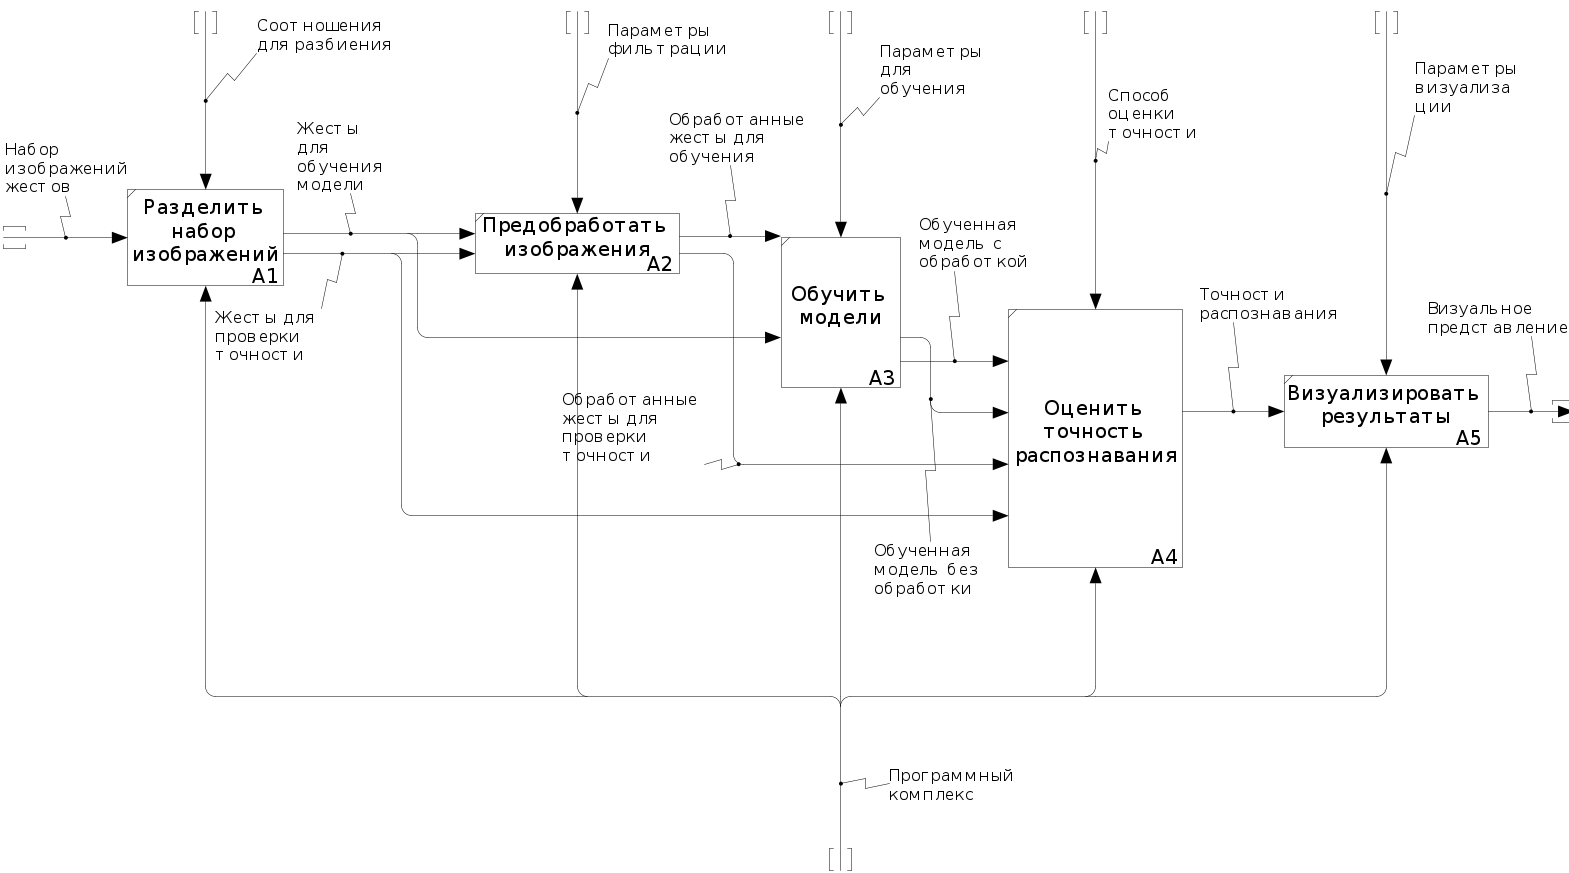
\includegraphics[width=\textwidth]{inc/img/research}
	\caption{Формальная модель эксперимента}
	\label{res:research}
\end{figure}

В качестве метрики качества распознавания метода используется вероятность корректной классификации жестового символа (формула \ref{res:acc}).

\begin{equation}
\label{res:acc}
\text{Точность} = \frac{\text{Верные классификации}}{\text{Ложные классификации} + \text{Верные классификации}}
\end{equation}

Каждый набор изображений был разделен в соотношении 20\% для валидации, 64\% для обучения и 16\% для тестирования. 

Исследования проводились с использованием платформы Google Colaboratory, предоставляющая бесплатное выполнение файлов ipython notebook с использованием GPU и TPU. В рамках одной сессии предоставляется 25,51 Гб ОЗУ и 68,40 дискового пространства.

\section{Результаты исследований}

Результаты экспериментов были обобщены и виде графиков зависимости точности распознавания от числа итераций, которые представлены на рисунках \ref{res:asl}, \ref{res:rsl_oleg}.

\begin{figure}
	\centering
	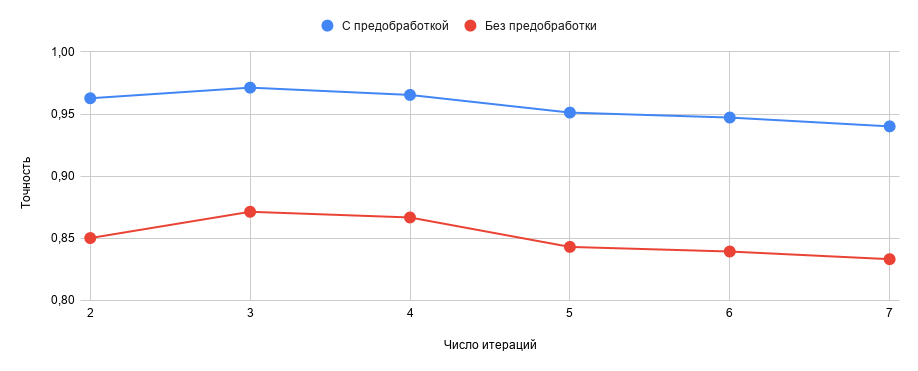
\includegraphics[width=0.8\textwidth]{inc/img/asl}
	\caption{Зависимость точности распознавания от предобработки входных данных и числе итераций на датасете ASL Finger Spelling Dataset}
	\label{res:asl}
\end{figure}


\begin{figure}
	\centering
	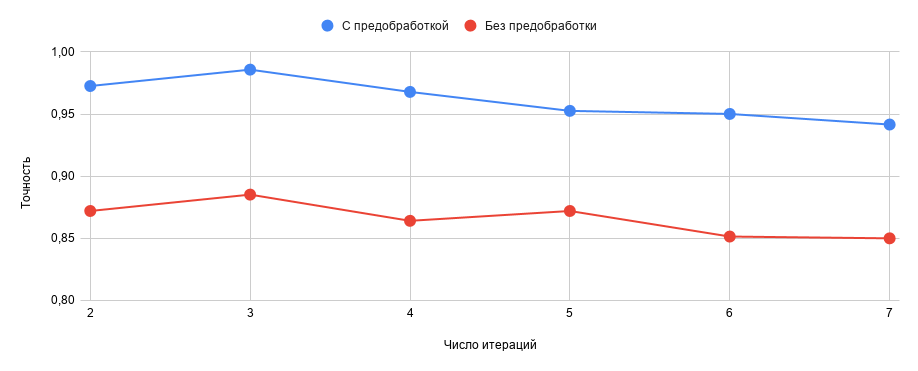
\includegraphics[width=0.9\textwidth]{inc/img/rsl_oleg}
	\caption{Зависимость точности распознавания от предобработки входных данных и числе итераций на датасете RSL by Oleg Potkin}
	\label{res:rsl_oleg}
\end{figure}

